\documentclass[aspectratio=169,12pt]{beamer}

\usepackage[utf8]{inputenc}
\usepackage[T5]{fontenc}
\usepackage[vietnamese]{babel}
\usepackage{lmodern}
\usepackage{graphicx}
\usepackage[dvipsnames]{xcolor}
\usepackage{booktabs}
\usepackage{tabularx}
\usepackage{array}
\usepackage{amsmath}
\usepackage{tcolorbox}

\graphicspath{{../report/artifacts/figures/}{../../figures/}}

% Bảng màu kế thừa từ mẫu slide của dự án.
\definecolor{primaryblue}{HTML}{0065BD}
\definecolor{secondaryblue}{HTML}{4A90E2}
\definecolor{accentorange}{HTML}{FF6B35}
\definecolor{darkgray}{HTML}{2C3E50}
\definecolor{lightgray}{HTML}{ECF0F1}
\definecolor{boxframe}{HTML}{009688}
\definecolor{successgreen}{HTML}{18864B}
\definecolor{mutedgray}{HTML}{6B7280}

\mode<presentation>{
  \usetheme{default}
  \useinnertheme{circles}
  \setbeamercovered{transparent}
}

\setbeamercolor{structure}{fg=primaryblue}
\setbeamercolor{frametitle}{bg=primaryblue,fg=white}
\setbeamercolor{title}{fg=primaryblue}
\setbeamercolor{normal text}{fg=darkgray,bg=white}
\setbeamerfont{frametitle}{size=\large,series=\bfseries}
\setbeamerfont{title}{size=\LARGE,series=\bfseries}
\setbeamerfont{subtitle}{size=\large}

\newif\ifappendixslides
\appendixslidesfalse

\setbeamertemplate{navigation symbols}{}
\setbeamertemplate{footline}{%
  \leavevmode
  \hbox{%
    \begin{beamercolorbox}[wd=.78\paperwidth,ht=2.8ex,dp=1.2ex,leftskip=4mm]{author in head/foot}%
      \scriptsize\textcolor{mutedgray}{Lab 2 -- Decision Tree Modeling and Improvement}
    \end{beamercolorbox}%
    \begin{beamercolorbox}[wd=.22\paperwidth,ht=2.8ex,dp=1.2ex,rightskip=4mm plus1fil]{date in head/foot}%
      \scriptsize\textcolor{darkgray}{%
        \ifappendixslides Appendix A\insertframenumber/4\else\insertframenumber/15\fi}
    \end{beamercolorbox}%
  }
}

\setlength{\tabcolsep}{5pt}
\renewcommand{\arraystretch}{1.18}
\newcolumntype{Y}{>{\raggedright\arraybackslash}X}
\newcolumntype{C}[1]{>{\centering\arraybackslash}p{#1}}
\newcolumntype{L}[1]{>{\raggedright\arraybackslash}p{#1}}

\tcbset{
  focusbox/.style={
    colframe=boxframe,
    colback=white,
    coltext=darkgray,
    boxrule=1.5pt,
    arc=3mm,
    left=4mm,
    right=4mm,
    top=3mm,
    bottom=3mm
  },
  riskbox/.style={
    colframe=accentorange,
    colback=white,
    coltext=darkgray,
    boxrule=1.3pt,
    arc=2.5mm,
    left=3mm,
    right=3mm,
    top=2mm,
    bottom=2mm
  },
  resultbox/.style={
    colframe=boxframe,
    colback=white,
    coltext=darkgray,
    boxrule=1.5pt,
    arc=2.5mm,
    left=3mm,
    right=3mm,
    top=2mm,
    bottom=2mm
  }
}

\newcommand{\metric}[3]{%
  \begin{minipage}[t]{0.30\linewidth}
    \centering
    {\Large\bfseries\textcolor{#1}{#2}}\\[-0.15em]
    {\small #3}
  \end{minipage}%
}

\newcommand{\sourcefooter}[1]{%
  \begin{tikzpicture}[remember picture,overlay]
    \node[
      anchor=south west,
      text=mutedgray,
      font=\tiny,
      inner sep=0pt,
      text width=0.78\paperwidth,
      align=left
    ] at ([xshift=4mm,yshift=4.4ex]current page.south west) {Nguồn: #1};
  \end{tikzpicture}%
}

\newcommand{\chaptertag}[2]{%
  \vspace{-0.16cm}%
  {\scriptsize\bfseries\textcolor{boxframe}{#1\enspace |\enspace #2}}\par
  \vspace{0.12cm}%
}

\title{Decision Tree Modeling\\and Improvement}
\subtitle{Từ cây cơ sở đến Cost-Complexity Pruning và Hierarchical Shrinkage}
\author{Nhóm thực hiện}
\institute{TRƯỜNG ĐẠI HỌC KHOA HỌC TỰ NHIÊN -- ĐHQG TP.HCM\\
KHOA CÔNG NGHỆ THÔNG TIN}
\date{Tháng 8 năm 2026}

\begin{document}

% 1 ---------------------------------------------------------------------------
\begin{frame}[plain]
  \begin{center}
    \vspace{0.35cm}
    {\LARGE\bfseries\textcolor{primaryblue}{Decision Tree Modeling}}\\[0.08cm]
    {\LARGE\bfseries\textcolor{primaryblue}{and Improvement}}\\[0.35cm]
    {\large Từ cây cơ sở đến CCP và Hierarchical Shrinkage}\\[0.55cm]
    {\color{primaryblue}\rule{0.74\textwidth}{1.2pt}}\\[0.55cm]
    {\normalsize\textbf{Nhóm thực hiện}}\\[0.18cm]
    {\small [HỌ TÊN -- MSSV] \quad [HỌ TÊN -- MSSV]}\\[0.08cm]
    {\small [HỌ TÊN -- MSSV] \quad [HỌ TÊN -- MSSV]}\\[0.55cm]
    {\small Introduction to Artificial Intelligence -- Lab 2}\\[0.1cm]
    {\scriptsize Trường Đại học Khoa học Tự nhiên -- ĐHQG TP.HCM}
  \end{center}
  \note{[Sources] Lab 2 assignment and project report.\\
  Talk track (0:20): Giới thiệu ngắn tên đề tài và mục tiêu: hiểu cây, đo đúng, rồi cải tiến có kiểm chứng.}
\end{frame}

% 2 ---------------------------------------------------------------------------
\begin{frame}
  \frametitle{Sáu chương nối từ vấn đề đến bằng chứng}
  \small
  \begin{enumerate}
    \item \textbf{Bối cảnh và động lực} -- vì sao cây sâu cần được kiểm soát?
    \item \textbf{Các công trình liên quan} -- CART, pruning và shrinkage đã giải quyết điều gì?
    \item \textbf{Kiến thức nền tảng} -- cây chọn split và suy luận như thế nào?
    \item \textbf{Phương pháp nghiên cứu} -- dữ liệu, protocol và cấu hình cải tiến.
    \item \textbf{Thực nghiệm và phân tích kết quả} -- hiệu năng, overfitting và độ phức tạp.
    \item \textbf{Kết luận} -- khi nào CCP + HS là lựa chọn hợp lý?
  \end{enumerate}
  \vspace{0.25cm}
  \begin{tcolorbox}[focusbox,width=0.90\textwidth,top=2mm,bottom=2mm]
    \centering
    Mạch trình bày đi từ \textbf{lý do nghiên cứu} đến \textbf{cơ chế}, rồi mới dùng thực nghiệm để trả lời ba câu hỏi nghiên cứu.
  \end{tcolorbox}
  \note{[Sources] Cấu trúc nghiên cứu của báo cáo nhóm.\\
  Talk track (0:35): Giới thiệu sáu chương như một mạch lập luận, không đọc chi tiết từng mục. Nhấn mạnh phần thực nghiệm chỉ có ý nghĩa sau khi protocol và cơ chế đã rõ.}
\end{frame}

% 3 ---------------------------------------------------------------------------
\begin{frame}
  \frametitle{Cây dễ giải thích, nhưng cây sâu rất dễ overfit}
  \chaptertag{1}{BỐI CẢNH VÀ ĐỘNG LỰC}
  \begin{tcolorbox}[riskbox,width=0.92\textwidth,top=2mm,bottom=2mm]
    \centering
    \textbf{Một cây không giới hạn có thể ghi nhớ tập train, tạo hàng chục nghìn lá và dự đoán quá tự tin ở các nhánh ít mẫu.}
  \end{tcolorbox}
  \vspace{0.22cm}
  \begin{enumerate}
    \item \textbf{RQ1 -- Phù hợp dữ liệu:} cây đơn hoạt động thế nào trên dữ liệu đa lớp, ảnh và dữ liệu bảng lớn?
    \item \textbf{RQ2 -- So sánh mô hình:} khi nào Decision Tree cạnh tranh được với RF, SVM và KNN?
    \item \textbf{RQ3 -- Cải tiến:} regularization có giảm overfitting mà vẫn giữ hiệu năng và khả năng diễn giải không?
  \end{enumerate}
  \sourcefooter{Breiman et al. (1984); mục tiêu nghiên cứu của nhóm.}
  \note{[Sources] Breiman et al., Classification and Regression Trees, 1984; report Chapter 1.\\
  Talk track (0:55): Mở bằng tension giữa diễn giải và overfitting. Ba RQ lần lượt hỏi về phạm vi phù hợp, đối chứng mô hình và giá trị của cải tiến.}
\end{frame}

% 4 ---------------------------------------------------------------------------
\begin{frame}
  \frametitle{Nghiên cứu trước giảm phương sai theo ba hướng bổ sung}
  \chaptertag{2}{CÁC CÔNG TRÌNH LIÊN QUAN}
  \scriptsize
  \begin{tabularx}{\textwidth}{@{}L{2.45cm}L{2.65cm}Y Y@{}}
    \toprule
    \textbf{Hướng nghiên cứu} & \textbf{Đại diện} & \textbf{Đóng góp} & \textbf{Điểm nhóm kế thừa} \\
    \midrule
    Cây phân loại & CART -- Breiman et al. (1984) & Split tham lam bằng impurity; luật if--then & Baseline và Cost-Complexity Pruning \\
    Dừng sớm/cắt tỉa & Pre-pruning; CCP & Giới hạn topology để giảm phương sai & So sánh dừng sớm với cắt cây sau khi fit \\
    Làm mượt dự đoán & Hierarchical Shrinkage -- Agarwal et al. (2022) & Kéo ước lượng nút con về nút cha & Kiểm tra HS riêng và kết hợp với CCP \\
    Mô hình đối chứng & Random Forest; SVM; KNN & Ensemble, kernel và lân cận cho ranh giới khác nhau & Đặt Decision Tree trong bối cảnh rộng hơn \\
    \bottomrule
  \end{tabularx}
  \vspace{0.22cm}
  \begin{tcolorbox}[focusbox,width=0.94\textwidth,top=1.5mm,bottom=1.5mm]
    \centering
    \textbf{Khoảng trống nhóm kiểm tra:} CCP + HS có tạo cây gọn hơn và giảm gap mà vẫn giữ macro-F1 trên dữ liệu đa lớp quy mô lớn hay không?
  \end{tcolorbox}
  \sourcefooter{Breiman et al. (1984, 2001); Cortes \& Vapnik (1995); Agarwal et al. (2022).}
  \note{[Sources] Breiman et al., CART, 1984; Breiman, Random Forests, 2001; Cortes and Vapnik, 1995; Agarwal et al., Hierarchical Shrinkage, 2022.\\
  Talk track (1:00): Không đọc như danh mục tài liệu. Chỉ ra ba hướng giảm phương sai: dừng sớm, cắt topology và làm mượt prediction; nghiên cứu của nhóm đặt chúng trong cùng protocol.}
\end{frame}

% 5 ---------------------------------------------------------------------------
\begin{frame}
  \frametitle{CART chọn phép chia làm giảm độ hỗn tạp lớn nhất}
  \chaptertag{3}{KIẾN THỨC NỀN TẢNG}
  \begin{columns}[T,onlytextwidth]
    \column{0.57\textwidth}
      \begin{tcolorbox}[focusbox,top=2mm,bottom=2mm]
        \centering
        \textbf{Gini impurity}\\[0.16cm]
        $\displaystyle Gini(S)=1-\sum_{k=1}^{K}p_k^2$\\[0.28cm]
        \textbf{Information gain của split $(j,t)$}\\[0.16cm]
        $\displaystyle \Delta G(j,t)=Gini(S)
        -\frac{n_L}{n}Gini(S_L)
        -\frac{n_R}{n}Gini(S_R)$
      \end{tcolorbox}
      \vspace{0.18cm}
      \centering
      $(j^\star,t^\star)=\arg\max_{j,t}\Delta G(j,t)$
    \column{0.40\textwidth}
      \textbf{Ý nghĩa}
      \begin{itemize}
        \item $p_k$: tỷ lệ lớp $k$ tại nút.
        \item Gain lớn: hai nút con thuần hơn nút cha.
        \item Mỗi đường từ gốc đến lá tạo một luật \textit{if--then}.
      \end{itemize}
      \textbf{Hệ quả}
      \begin{itemize}
        \item Split tham lam, theo từng trục.
        \item Cây sâu có phương sai cao.
      \end{itemize}
  \end{columns}
  \sourcefooter{CART: Breiman et al. (1984).}
  \note{[Sources] Breiman et al., 1984.\\
  Talk track (1:05): Giải thích Gini bằng xác suất lớp, sau đó đọc gain như phần impurity giảm đi sau split. Kết nối split tham lam với nguy cơ overfitting ở phần sau.}
\end{frame}

% 6 ---------------------------------------------------------------------------
\begin{frame}
  \frametitle{Huấn luyện lặp đệ quy; suy luận chỉ đi theo một nhánh}
  \chaptertag{3}{KIẾN THỨC NỀN TẢNG}
  \begin{tcolorbox}[focusbox,width=0.94\textwidth,top=2mm,bottom=2mm]
    \begin{columns}[T,onlytextwidth]
      \column{0.57\textwidth}
        \textbf{Pseudocode huấn luyện}\\[0.12cm]
        {\small\ttfamily
        BuildTree($S$):\\
        \quad if Stop($S$): return Leaf($\hat p(y\mid S)$)\\
        \quad $(j^\star,t^\star)\leftarrow\arg\max_{j,t}\Delta G(j,t)$\\
        \quad $S_L,S_R\leftarrow$ Split($S,j^\star,t^\star$)\\
        \quad return Node($j^\star,t^\star$,\\
        \qquad BuildTree($S_L$), BuildTree($S_R$))}
      \column{0.39\textwidth}
        \textbf{Pseudocode dự đoán}\\[0.12cm]
        {\small\ttfamily
        Predict($x,v$):\\
        \quad while $v$ is not leaf:\\
        \qquad $v\leftarrow$ left if $x_j\leq t$\\
        \qquad else right\\
        \quad return $\arg\max_k\hat p_k(v)$}
    \end{columns}
  \end{tcolorbox}
  \vspace{0.12cm}
  \begin{center}
    \textcolor{accentorange}{\textbf{Nơi regularization can thiệp:}}
    điều kiện dừng, topology sau khi fit hoặc xác suất dự đoán tại các nút.
  \end{center}
  \sourcefooter{Pseudocode tổng quát hóa từ thuật toán CART.}
  \note{[Sources] Breiman et al., 1984; scikit-learn DecisionTreeClassifier documentation.\\
  Talk track (1:00): Theo dõi một vòng đệ quy: thử split, chọn gain lớn nhất, gọi lại cho hai nhánh. Khi dự đoán, mỗi mẫu chỉ đi một đường; ba cải tiến sẽ can thiệp vào ba vị trí khác nhau.}
\end{frame}

% 7 ---------------------------------------------------------------------------
\begin{frame}
  \frametitle{Ba dataset tạo ra ba điều kiện kiểm thử khác nhau}
  \chaptertag{4}{PHƯƠNG PHÁP NGHIÊN CỨU}
  \small
  \setlength{\tabcolsep}{3.5pt}
  \begin{tabularx}{\textwidth}{@{}L{2.65cm}C{1.55cm}C{1.60cm}C{1.0cm}Y@{}}
    \toprule
    \textbf{Dataset} & \textbf{Mẫu} & \textbf{Features} & \textbf{Lớp} & \textbf{Vai trò} \\
    \midrule
    Letter Recognition & 18.668 & 16 & 26 & Stress test đa lớp với đặc trưng hình học \\
    Handwritten Digits & 1.797 & 64 & 10 & Stress test dữ liệu ảnh ít mẫu, nhiều chiều \\
    \textcolor{primaryblue}{\textbf{Covertype}} & \textcolor{primaryblue}{\textbf{581.012}} & \textcolor{primaryblue}{\textbf{54}} & \textcolor{primaryblue}{\textbf{7}} & \textcolor{primaryblue}{\textbf{Dataset chính: dữ liệu bảng lớn, mất cân bằng}} \\
    \bottomrule
  \end{tabularx}
  \vspace{0.14cm}
  \begin{tcolorbox}[focusbox,width=0.92\textwidth,top=1.2mm,bottom=1.2mm]
    \centering
    \textbf{Covertype trả lời yêu cầu chính của đề;} Letter và Digits kiểm tra độ bền của kết luận trên cấu trúc dữ liệu khác.
  \end{tcolorbox}
  \sourcefooter{UCI Letter Recognition; scikit-learn Digits; UCI Covertype.}
  \note{[Sources] UCI Letter Recognition DOI 10.24432/C5ZP40; sklearn load_digits; UCI Covertype DOI 10.24432/C50K5N.\\
  Talk track (0:50): Covertype là dataset chính. Hai bộ nhỏ là stress test, không phải ba bài toán độc lập có trọng số ngang nhau.}
\end{frame}

% 8 ---------------------------------------------------------------------------
\begin{frame}
  \frametitle{Một protocol chung giúp so sánh công bằng}
  \chaptertag{4}{PHƯƠNG PHÁP NGHIÊN CỨU}
  \begin{tcolorbox}[focusbox,width=0.94\textwidth,top=2mm,bottom=2mm]
    \centering
    \textbf{Dữ liệu sạch} $\longrightarrow$ \textbf{80/20 stratified split}
    $\longrightarrow$ \textbf{train} $\longrightarrow$ \textbf{test cuối cùng}\\[0.28cm]
    \texttt{random\_state=42} \quad $\vert$ \quad scaler chỉ fit trên train cho SVM/KNN
    \quad $\vert$ \quad CV chỉ dùng tập train
  \end{tcolorbox}
  \vspace{0.25cm}
  \begin{columns}[T,onlytextwidth]
    \column{0.49\textwidth}
      \textbf{Chất lượng dự đoán}
      \begin{itemize}
        \item Accuracy và Error rate
        \item Macro-F1, confusion matrix
        \item Train--test gap
      \end{itemize}
    \column{0.49\textwidth}
      \textbf{Hiệu quả và độ phức tạp}
      \begin{itemize}
        \item Fit/prediction time
        \item Độ sâu và số lá
        \item 3-fold CV chọn tham số
      \end{itemize}
  \end{columns}
  \sourcefooter{Protocol dùng chung của năm notebook; test set không tham gia chọn siêu tham số.}
  \note{[Sources] Project notebooks and report Chapter 3.\\
  Talk track (0:55): Nhấn mạnh không data leakage. Macro-F1 cần thiết cho Covertype mất cân bằng; gap và số lá giúp đánh giá regularization thay vì chỉ nhìn accuracy.}
\end{frame}

% 9 ---------------------------------------------------------------------------
\begin{frame}
  \frametitle{CCP đổi topology, HS làm mượt xác suất dự đoán}
  \chaptertag{4}{PHƯƠNG PHÁP NGHIÊN CỨU}
  \small
  \textbf{Pre-pruning.} Dừng sớm bằng \texttt{max\_depth} hoặc \texttt{min\_samples\_leaf}.\\[0.18cm]
  \textbf{Cost-Complexity Pruning.}
  \[
    T_\alpha=\arg\min_{T\subseteq T_0}\left[R(T)+\alpha\,|\mathcal{L}(T)|\right]
  \]
  \textbf{Hierarchical Shrinkage.}
  \[
    \hat p_{HS}(v)=\hat p_{HS}(pa(v))+
    \frac{n_v}{n_v+\lambda}\left[\hat p(v)-\hat p(pa(v))\right]
  \]
  \vspace{-0.12cm}
  \begin{tcolorbox}[focusbox,width=0.94\textwidth,top=1.5mm,bottom=1.5mm]
    \centering
    E0 Baseline \quad E1 Pre-pruning \quad E2 CCP \quad E3 HS \quad
    \textbf{\textcolor{boxframe}{E4 CCP + HS}}\\[0.1cm]
    $\alpha$ và $\lambda$ được chọn bằng 3-fold CV chỉ trên tập train.
  \end{tcolorbox}
  \sourcefooter{Breiman et al. (1984); Agarwal et al. (2022); cấu hình benchmark của nhóm.}
  \note{[Sources] Breiman et al., 1984; Agarwal et al., Hierarchical Shrinkage, 2022; HS benchmark notebook.\\
  Talk track (1:20): Pre-pruning tác động trước khi cây hoàn tất, CCP chọn subtree sau khi fit, HS giữ nguyên split nhưng co xác suất nút con về cha. E4 kết hợp cắt topology và làm mượt prediction.}
\end{frame}

% 10 --------------------------------------------------------------------------
\begin{frame}
  \frametitle{Không có mô hình tốt nhất trên mọi dataset}
  \chaptertag{5}{THỰC NGHIỆM VÀ PHÂN TÍCH KẾT QUẢ}
  \small
  \renewcommand{\arraystretch}{1.08}
  \begin{tabularx}{\textwidth}{@{}L{2.8cm}L{2.4cm}C{1.7cm}C{1.7cm}Y@{}}
    \toprule
    \textbf{Dataset} & \textbf{Mô hình tốt nhất} & \textbf{Accuracy} & \textbf{Macro-F1} & \textbf{Diễn giải} \\
    \midrule
    Letter Recognition & \textcolor{primaryblue}{\textbf{Random Forest}} & \textbf{95,13\%} & \textbf{95,12\%} & Ensemble giảm phương sai của cây đơn \\
    Handwritten Digits & \textcolor{primaryblue}{\textbf{SVM--RBF}} & \textbf{97,22\%} & \textbf{97,18\%} & Kernel phù hợp ranh giới ảnh nhiều chiều \\
    Covertype & \textcolor{boxframe}{\textbf{Decision Tree}} & \textbf{93,89\%} & \textbf{90,34\%} & Cây khai thác hiệu quả dữ liệu bảng lớn \\
    \bottomrule
  \end{tabularx}
  \vspace{0.06cm}
  \begin{tcolorbox}[focusbox,width=0.92\textwidth,top=1mm,bottom=1mm]
    \centering
    \textbf{Cấu trúc dữ liệu quyết định mô hình phù hợp;} kết quả chỉ áp dụng cho backend và siêu tham số đã khảo sát.
  \end{tcolorbox}
  \sourcefooter{Notebook so sánh 3 dataset $\times$ 4 model; cùng train/test split.}
  \note{[Sources] gpu_three_dataset_four_model_comparison summary.\\
  Talk track (1:10): RF thắng Letter, SVM thắng Digits, cây đơn thắng Covertype trong cấu hình này. Không suy rộng thành thứ hạng thuật toán phổ quát.}
\end{frame}

% 11 --------------------------------------------------------------------------
\begin{frame}
  \frametitle{Baseline Covertype dự đoán tốt nhưng tạo cây rất lớn}
  \chaptertag{5}{THỰC NGHIỆM VÀ PHÂN TÍCH KẾT QUẢ}
  \begin{center}
    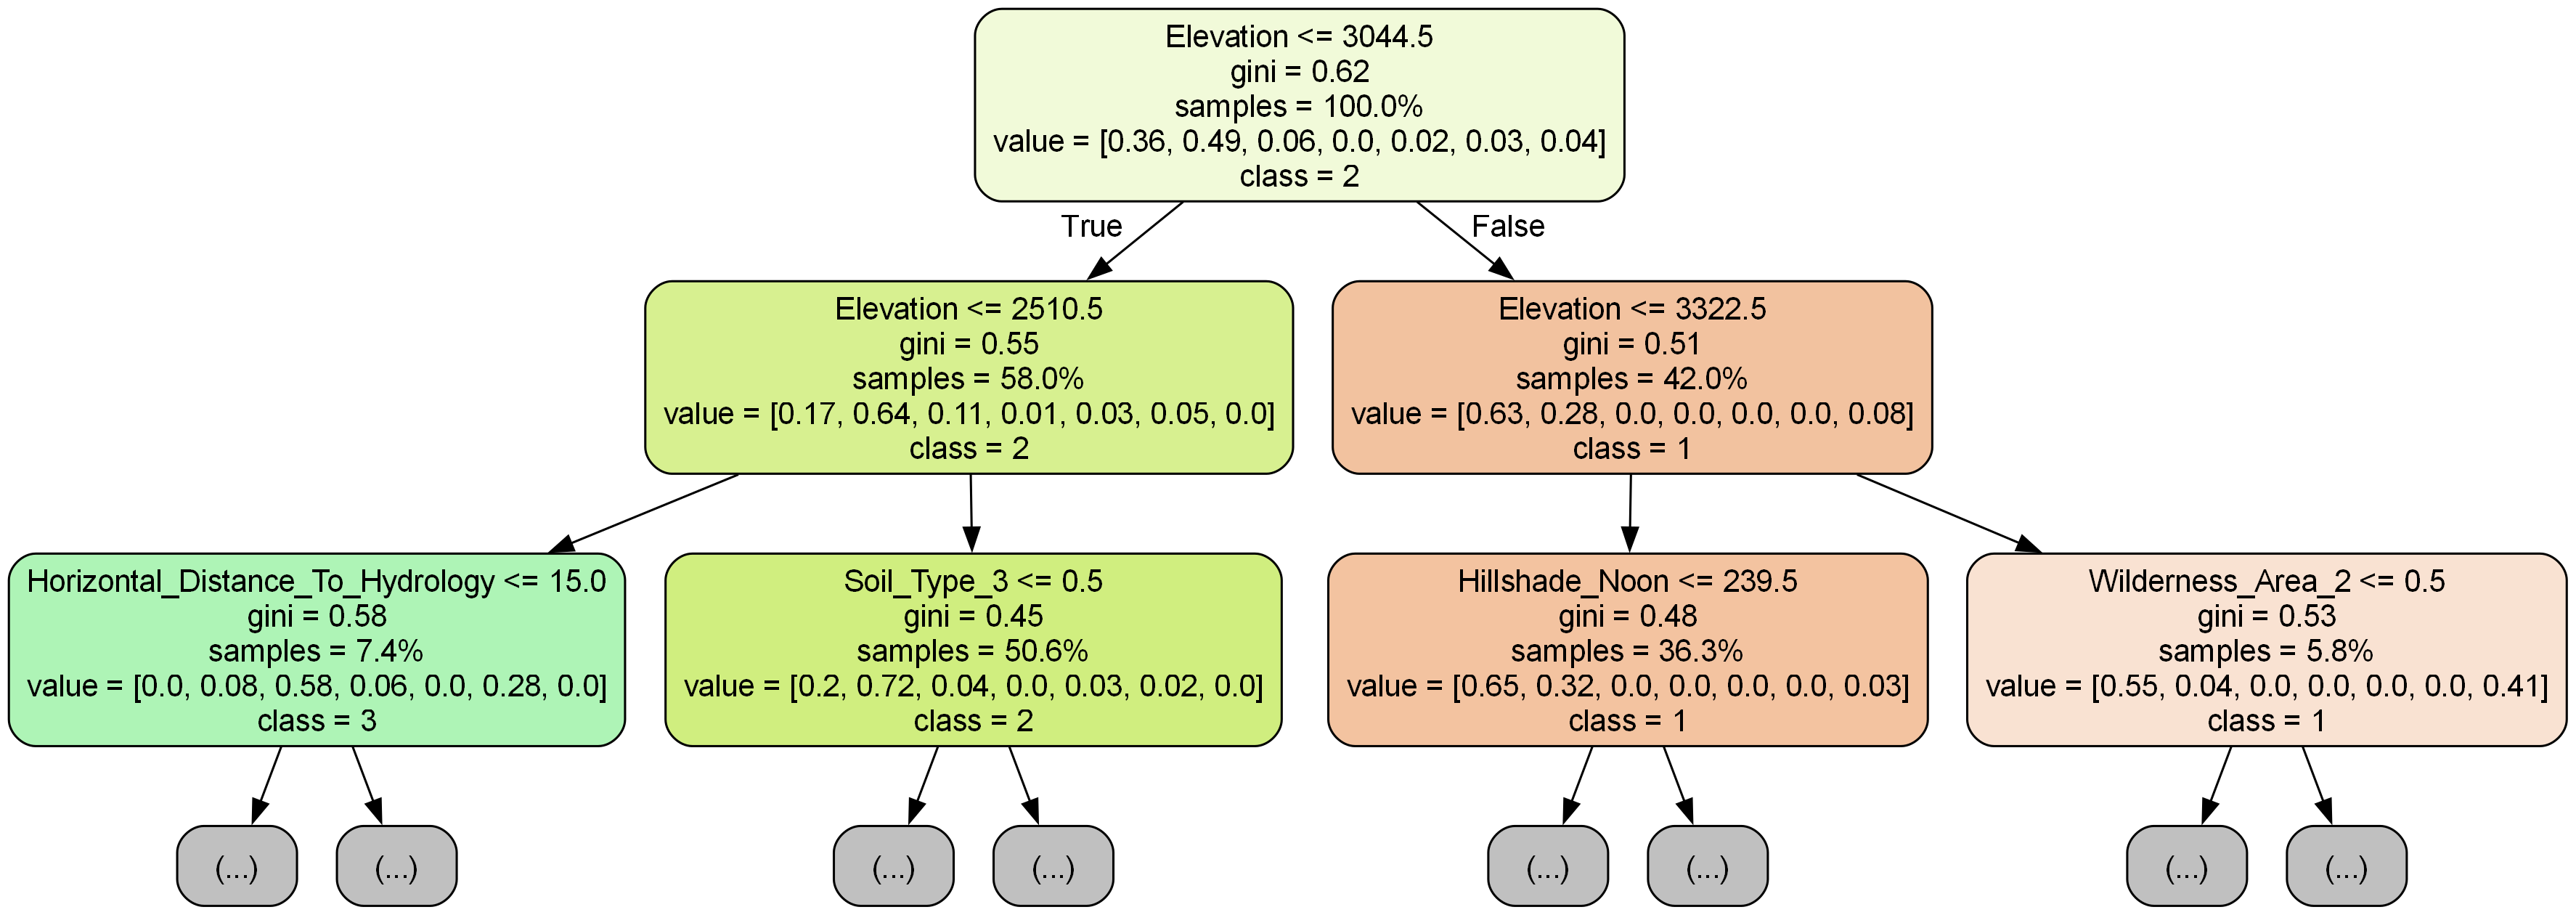
\includegraphics[width=0.92\linewidth,height=0.36\textheight,keepaspectratio]{dt_covertype_baseline__tree_top_levels.png}
  \end{center}
  \vspace{-0.12cm}
  \begin{center}
    \metric{primaryblue}{93,89\%}{Accuracy}\hfill
    \metric{accentorange}{6,11\%}{Error rate}\hfill
    \metric{boxframe}{90,34\%}{Macro-F1}
  \end{center}
  \vspace{-0.16cm}
  {\scriptsize\textbf{Luật:} \texttt{Elevation $\leq$ 3044,5} $\rightarrow$ nhánh lớp 2. \textbf{Độ phức tạp:} depth = 41; leaves = 23.956.}
  \sourcefooter{Baseline CART trên Covertype; hình chỉ hiển thị 3 tầng đầu.}
  \note{[Sources] dt_covertype_scalability baseline result; tree exported with scikit-learn 1.6.1.\\
  Talk track (1:00): Đọc một split thật để chứng minh tính diễn giải. Sau đó đối chiếu với 23.956 lá: giải thích cục bộ được, nhưng toàn cây quá lớn để kiểm soát.}
\end{frame}

% 12 --------------------------------------------------------------------------
\begin{frame}
  \frametitle{Generalization gap xác nhận cây baseline đang overfit}
  \chaptertag{5}{THỰC NGHIỆM VÀ PHÂN TÍCH KẾT QUẢ}
  \begin{center}
    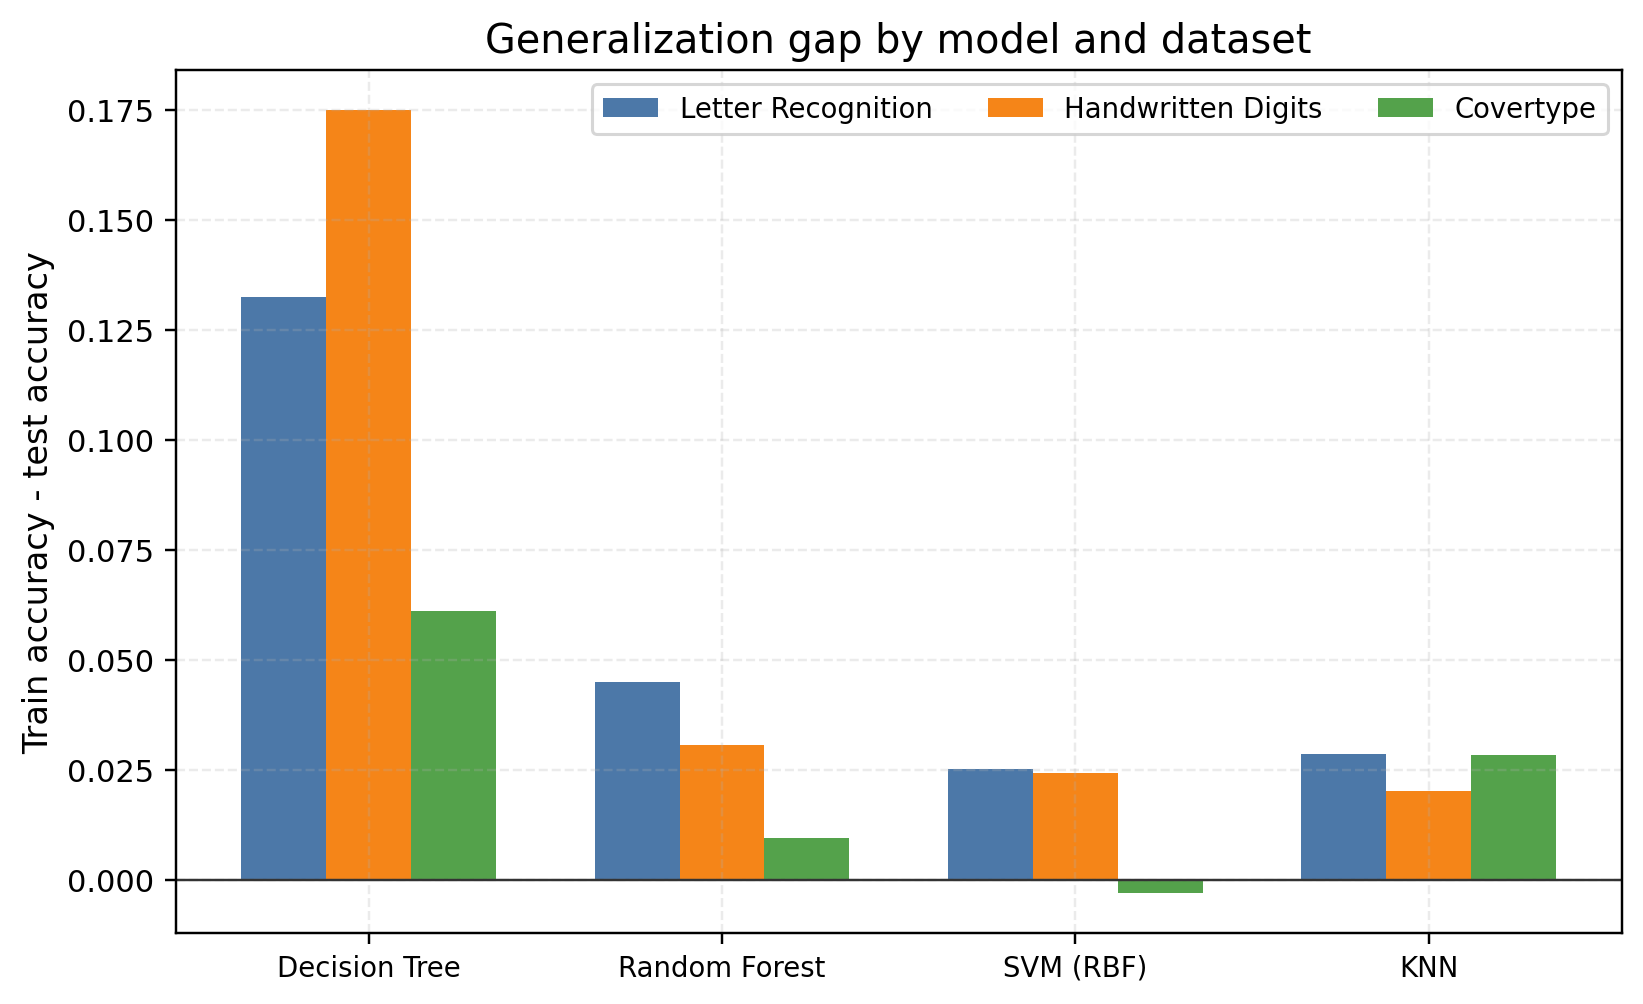
\includegraphics[width=0.80\linewidth,height=0.46\textheight,keepaspectratio]{report_model_generalization_gap.png}
  \end{center}
  \vspace{-0.10cm}
  \begin{tcolorbox}[riskbox,width=0.90\textwidth,top=1.2mm,bottom=1.2mm]
    \centering
    Covertype đạt \textbf{100\% train accuracy} nhưng chỉ \textbf{93,89\% test accuracy}: gap \textbf{6,11 điểm \%}.
  \end{tcolorbox}
  \sourcefooter{Train accuracy đo trên mẫu chẩn đoán cố định; test accuracy đo trên toàn bộ test set.}
  \note{[Sources] Model comparison summary and report generalization-gap figure.\\
  Talk track (0:45): Test accuracy cao không loại trừ overfitting. Gap cùng số lá lớn tạo bằng chứng để đánh giá các phương pháp regularization.}
\end{frame}

% 13 --------------------------------------------------------------------------
\begin{frame}
  \frametitle{HS đạt accuracy cao nhất, CCP + HS đạt macro-F1 tốt nhất}
  \chaptertag{5}{THỰC NGHIỆM VÀ PHÂN TÍCH KẾT QUẢ}
  \scriptsize
  \begin{tabular}{@{}L{3.2cm}C{1.65cm}C{1.65cm}C{1.65cm}C{1.55cm}C{1.6cm}@{}}
    \toprule
    \textbf{Cấu hình} & \textbf{Accuracy} & \textbf{Error} & \textbf{Macro-F1} & \textbf{Depth} & \textbf{Leaves} \\
    \midrule
    E0 Baseline & 93,89\% & 6,11\% & 90,34\% & 41 & 23.956 \\
    E1 Pre-pruning & 92,97\% & 7,03\% & 88,85\% & 40 & 16.637 \\
    E2 CCP & 93,92\% & 6,08\% & 90,45\% & 39 & 16.361 \\
    \textcolor{primaryblue}{\textbf{E3 HS}} & \textcolor{primaryblue}{\textbf{93,97\%}} & \textcolor{primaryblue}{\textbf{6,03\%}} & 90,48\% & 41 & 23.956 \\
    \textcolor{boxframe}{\textbf{E4 CCP + HS}} & 93,93\% & 6,07\% & \textcolor{boxframe}{\textbf{90,53\%}} & \textbf{39} & \textbf{16.361} \\
    \bottomrule
  \end{tabular}
  \vspace{0.30cm}
  \begin{tcolorbox}[resultbox,width=0.92\textwidth,top=2mm,bottom=2mm]
    \centering
    Vì Covertype mất cân bằng, nhóm chọn \textbf{E4}: macro-F1 cao nhất, gap thấp hơn và cây nhỏ hơn E3.
  \end{tcolorbox}
  \sourcefooter{HS benchmark trên Covertype; 3-fold CV chọn tham số trên train.}
  \note{[Sources] dt_hierarchical_shrinkage summary and selection outputs.\\
  Talk track (1:05): E3 thắng accuracy, nhưng E4 là lựa chọn đa mục tiêu. Pre-pruning quá mạnh gây underfit; CCP một mình đã cải thiện nhẹ.}
\end{frame}

% 14 --------------------------------------------------------------------------
\begin{frame}
  \frametitle{CCP + HS cải thiện trade-off, không phải accuracy đơn thuần}
  \chaptertag{5}{THỰC NGHIỆM VÀ PHÂN TÍCH KẾT QUẢ}
  \begin{columns}[T,onlytextwidth]
    \column{0.61\textwidth}
      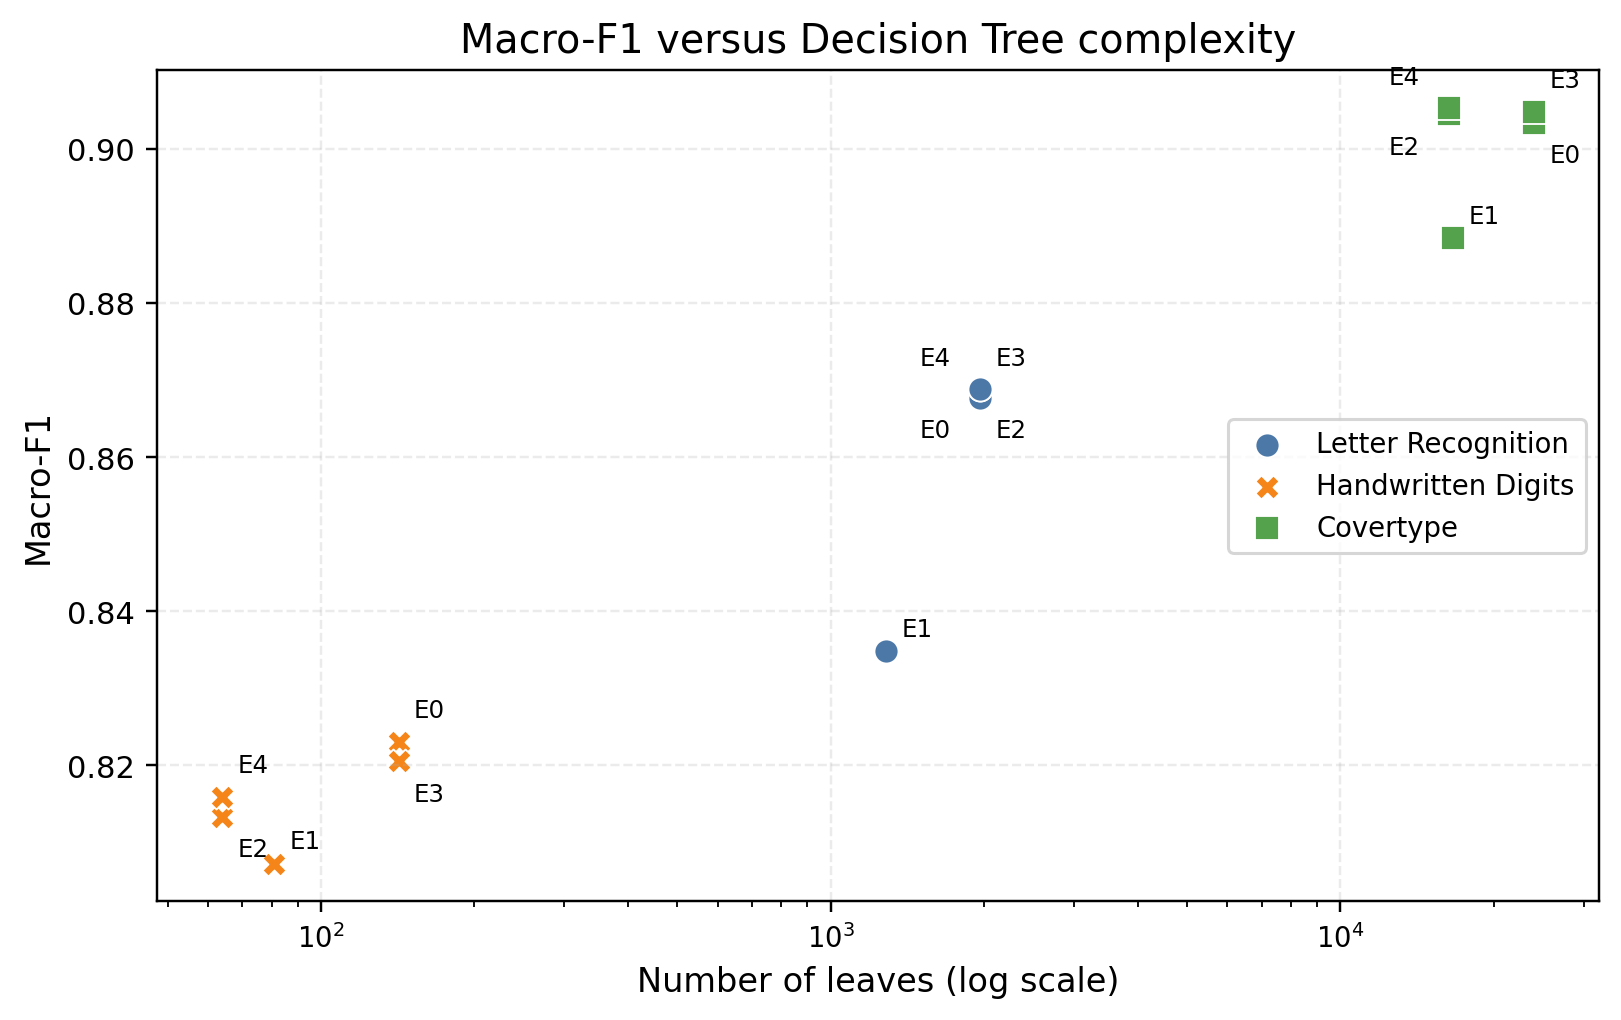
\includegraphics[width=\linewidth,height=0.48\textheight,keepaspectratio]{report_hs_performance_vs_complexity.png}
    \column{0.36\textwidth}
      \vspace{0.05cm}
      {\Large\bfseries\textcolor{boxframe}{$-31,7\%$}}\\[-0.1cm]
      {\small số lá: 23.956 $\rightarrow$ 16.361}\\[0.18cm]
      {\Large\bfseries\textcolor{boxframe}{$-17,6\%$}}\\[-0.1cm]
      {\small gap: 6,11 $\rightarrow$ 5,04 điểm \%}\\[0.18cm]
      {\Large\bfseries\textcolor{primaryblue}{$+0,19$ điểm \%}}\\[-0.1cm]
      {\small macro-F1: 90,34\% $\rightarrow$ 90,53\%}
  \end{columns}
  \vspace{-0.08cm}
  \begin{tcolorbox}[resultbox,width=0.94\textwidth,top=1.3mm,bottom=1.3mm]
    \centering\small
    \textbf{Stress test:} Letter $+0,11$ điểm macro-F1; Digits $-0,71$; Covertype $+0,19$. Lợi ích rõ nhất khi dữ liệu và cây đủ lớn.
  \end{tcolorbox}
  \sourcefooter{So sánh E0--E4 trên ba dataset; Covertype có 116.203 mẫu test.}
  \note{[Sources] HS benchmark summaries across three datasets.\\
  Talk track (1:10): Giá trị lớn không nằm ở +0,05 điểm accuracy mà ở số lá và gap giảm đồng thời macro-F1 tăng. Digits là phản ví dụ cho thấy HS không phải thuốc tăng điểm phổ quát.}
\end{frame}

% 15 --------------------------------------------------------------------------
\begin{frame}
  \frametitle{Decision Tree phù hợp nhất khi cần cây gọn và diễn giải được}
  \chaptertag{6}{KẾT LUẬN}
  \vspace{0.05cm}
  \begin{tcolorbox}[focusbox,width=0.91\textwidth,top=2mm,bottom=2mm]
    \textbf{RQ1 -- Phù hợp dữ liệu:} cây đơn mạnh nhất trên Covertype, nhưng yếu hơn trên Letter và Digits.\\[0.28cm]
    \textbf{RQ2 -- So sánh mô hình:} không có thuật toán thắng mọi dataset; cấu trúc dữ liệu quyết định lựa chọn.\\[0.28cm]
    \textbf{RQ3 -- Cải tiến:} CCP + HS phù hợp khi cây sâu, dữ liệu lớn và cần cân bằng hiệu năng với khả năng diễn giải.
  \end{tcolorbox}
  \vspace{0.12cm}
  \centering
  {\normalsize\bfseries\textcolor{boxframe}{Cây tốt hơn không chỉ chính xác hơn -- mà còn gọn hơn, ít overfit hơn và vẫn giải thích được.}}\\[0.18cm]
  {\scriptsize\textcolor{mutedgray}{Phạm vi kết luận: một split chính; backend CPU/GPU khác nhau; chưa chứng minh HS luôn tốt hơn.}}
  \note{[Sources] Synthesis of all reported experiments and limitations.\\
  Talk track (0:40): Trả lời trực tiếp ba RQ, sau đó chốt bằng tiêu chí lựa chọn. Chủ động giới hạn phạm vi kết luận trước phần câu hỏi.}
\end{frame}

% APPENDIX --------------------------------------------------------------------
\appendix
\appendixslidestrue
\setcounter{framenumber}{0}

% A1 --------------------------------------------------------------------------
\begin{frame}
  \frametitle{Appendix: Kết quả đầy đủ của 3 dataset $\times$ 4 model}
  \scriptsize
  \begin{tabular}{@{}L{2.25cm}L{2.25cm}C{1.3cm}C{1.3cm}C{1.3cm}C{1.65cm}@{}}
    \toprule
    \textbf{Dataset} & \textbf{Model} & \textbf{Accuracy} & \textbf{Macro-F1} & \textbf{Error} & \textbf{Tổng time (s)} \\
    \midrule
    Letter & Decision Tree & 86,77\% & 86,77\% & 13,23\% & 0,084 \\
           & Random Forest & \textbf{95,13\%} & \textbf{95,12\%} & 4,87\% & 3,097 \\
           & SVM--RBF & 92,31\% & 92,32\% & 7,69\% & 3,707 \\
           & KNN & 94,08\% & 94,08\% & 5,92\% & 0,005 \\
    \addlinespace
    Digits & Decision Tree & 82,50\% & 82,30\% & 17,50\% & 0,021 \\
           & Random Forest & 96,94\% & 96,89\% & 3,06\% & 0,628 \\
           & SVM--RBF & \textbf{97,22\%} & \textbf{97,18\%} & 2,78\% & 0,718 \\
           & KNN & 96,39\% & 96,34\% & 3,61\% & 0,003 \\
    \addlinespace
    Covertype & Decision Tree & \textbf{93,89\%} & \textbf{90,34\%} & 6,11\% & 7,409 \\
              & Random Forest & 79,57\% & 65,86\% & 20,43\% & 2,995 \\
              & SVM--RBF & 79,07\% & 63,78\% & 20,93\% & 125,547 \\
              & KNN & 92,84\% & 87,32\% & 7,16\% & 5,756 \\
    \bottomrule
  \end{tabular}
  \par\vspace{0.15cm}
  \noindent\begin{minipage}{\textwidth}
    \tiny Runtime phản ánh backend và pipeline thực tế; không dùng để suy ra speedup phần cứng thuần túy.
  \end{minipage}
  \sourcefooter{gpu\_three\_dataset\_four\_model\_comparison\_summary.csv.}
  \note{[Sources] Full model comparison summary.\\
  Q&A: Nếu được hỏi vì sao RF Covertype thấp, nhấn mạnh cuML backend/cấu hình và giới hạn phạm vi kết luận.}
\end{frame}

% A2 --------------------------------------------------------------------------
\begin{frame}
  \frametitle{Appendix: Confusion matrix cho thấy lỗi tập trung ở lớp thiểu số}
  \begin{center}
    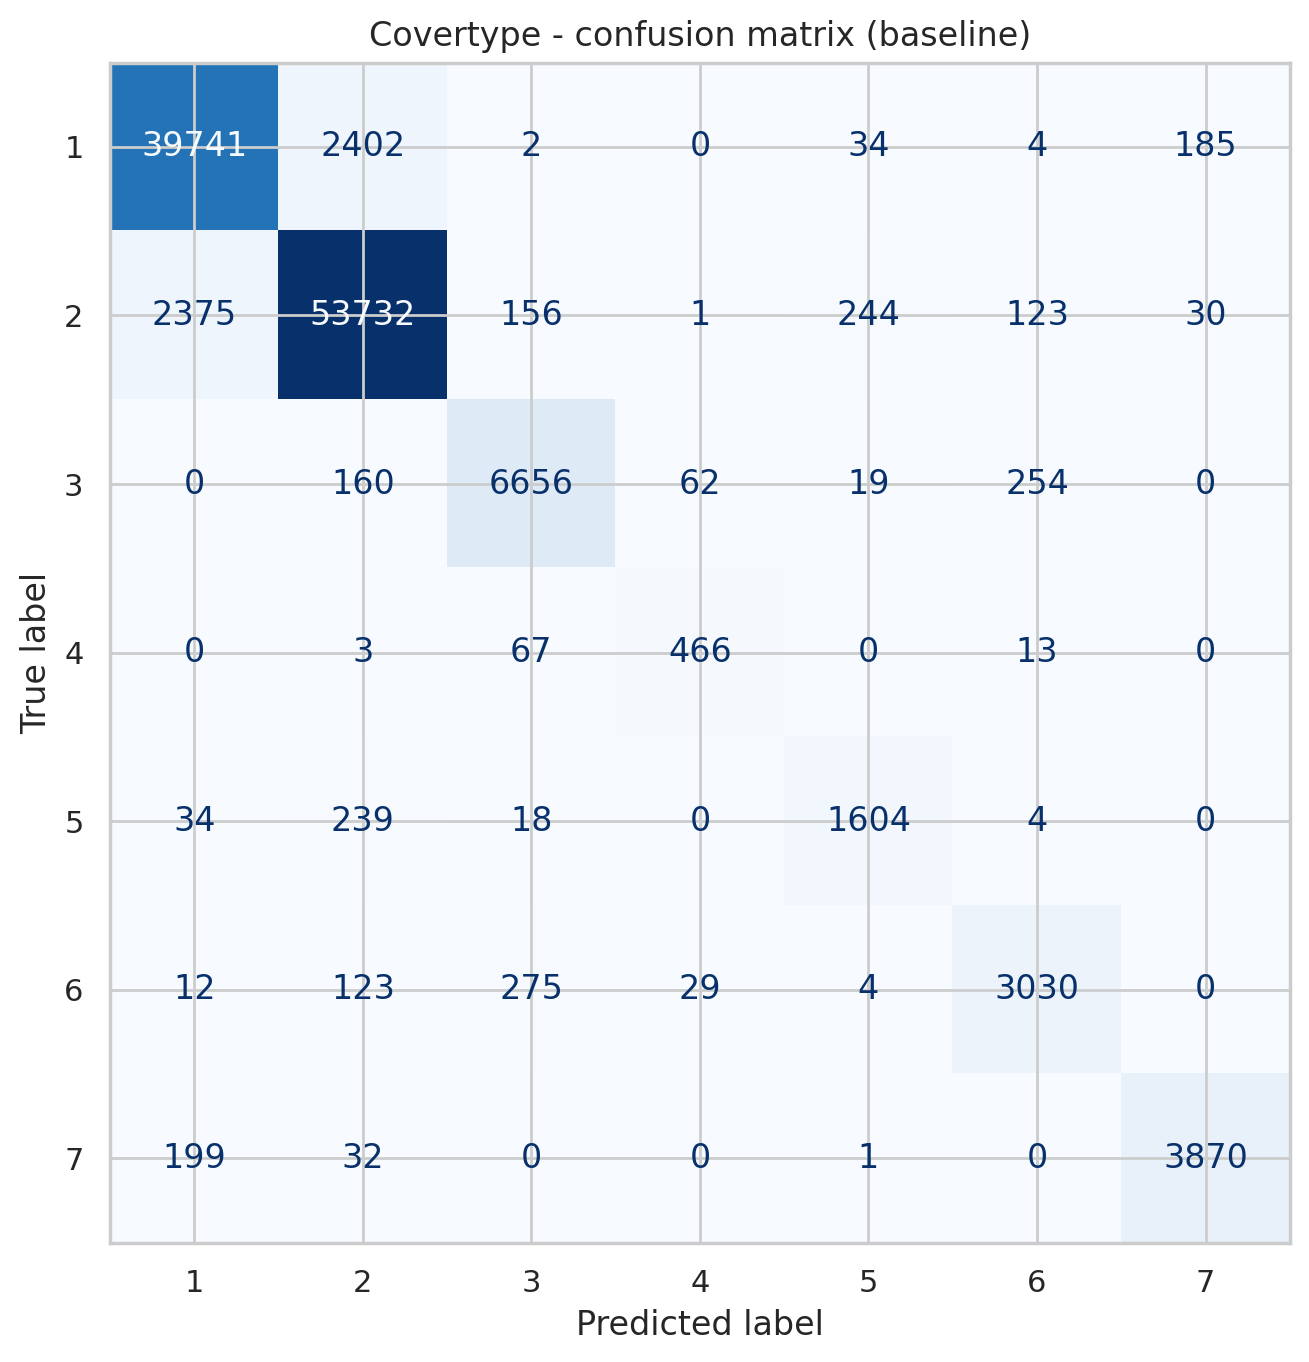
\includegraphics[width=0.68\linewidth,height=0.74\textheight,keepaspectratio]{dt_covertype_scalability__confusion_matrix.png}
  \end{center}
  \sourcefooter{Decision Tree baseline trên tập test Covertype.}
  \note{[Sources] Covertype baseline confusion matrix.\\
  Q&A: Accuracy bị chi phối bởi lớp lớn, vì vậy nhóm dùng macro-F1 để cho mỗi lớp trọng số ngang nhau.}
\end{frame}

% A3 --------------------------------------------------------------------------
\begin{frame}
  \frametitle{Appendix: Tham số cải tiến được chọn chỉ từ tập train}
  \small
  \begin{tabularx}{\textwidth}{@{}L{2.6cm}Y Y Y@{}}
    \toprule
    \textbf{Dataset} & \textbf{Pre-pruning} & \textbf{CCP} & \textbf{HS} \\
    \midrule
    Letter & \texttt{max\_depth=16} & $\alpha=0$ & $\lambda=10$ \\
    Digits & \texttt{max\_depth=8} & $\alpha=0{,}002196$ & $\lambda=10$ \\
    Covertype & \shortstack{\texttt{min\_samples\_leaf}\\=5} & $\alpha=3{,}442\times10^{-6}$ & $\lambda=10$ \\
    \bottomrule
  \end{tabularx}
  \vspace{0.45cm}
  \begin{tcolorbox}[focusbox,width=0.92\textwidth]
    \centering
    \textbf{3-fold cross-validation trên train} chọn cấu hình; test set chỉ được mở để báo cáo cuối cùng.
  \end{tcolorbox}
  \par\vspace{0.12cm}
  {\scriptsize 5-fold CV độc lập cho baseline Covertype: accuracy $0{,}9330\pm0{,}0011$; macro-F1 $0{,}8923\pm0{,}0011$.\par}
  \sourcefooter{HS CV selection; Covertype scalability cross-validation.}
  \note{[Sources] HS CV selection CSV; Covertype 5-fold CV output.\\
  Q&A: Một seed là hạn chế của holdout chính, nhưng baseline Covertype có độ lệch chuẩn nhỏ qua 5 fold.}
\end{frame}

% A4 --------------------------------------------------------------------------
\begin{frame}
  \frametitle{Appendix: Hardware, tài liệu và đóng góp nhóm}
  \small
  \textbf{Hardware/backend.} Kaggle GPU x2; cuML ghi nhận Tesla T4 cho RF/SVM/KNN. Decision Tree và HS dùng scikit-learn trên CPU; notebook baseline ghi nhận P100 khả dụng nhưng compute device vẫn là CPU.\\[0.35cm]

  \textbf{Tài liệu chính.} Breiman et al. (1984), \textit{Classification and Regression Trees}; Agarwal et al. (2022), \textit{Hierarchical Shrinkage}; UCI Letter Recognition và Covertype; scikit-learn Digits; RAPIDS cuML.\\[0.35cm]

  \textbf{Đóng góp thành viên.}
  \begin{tabularx}{\textwidth}{@{}L{3.4cm}Y@{}}
    {[HỌ TÊN -- MSSV]} & [Dữ liệu / baseline / kiểm thử] \\
    {[HỌ TÊN -- MSSV]} & [Benchmark model / Kaggle GPU] \\
    {[HỌ TÊN -- MSSV]} & [Hierarchical Shrinkage / phân tích] \\
    {[HỌ TÊN -- MSSV]} & [Report / slide / tổng hợp kết quả] \\
  \end{tabularx}
  \sourcefooter{Metadata notebook; tài liệu tham khảo trong report.}
  \note{[Sources] Notebook environment metadata; report references.\\
  Q&A: GPU x2 là cấu hình môi trường, không khẳng định hai GPU được dùng song song. Điền tên, MSSV và đóng góp thật trước khi nộp.}
\end{frame}

\end{document}
